\documentclass[a4paper,11pt,titlepage]{article}

\usepackage{ucs}
% per input encoding kann man Umlaute direkt einsetzten, aber  dann ist man von Font des jeweiligen Rechners abh"angig. Daher mag ich es nicht!
%\usepackage[utf8x]{inputenc}
\usepackage[german,ngerman]{babel}
\usepackage{fontenc}
\usepackage[pdftex]{graphicx}
%\usepackage{latexsym}
\usepackage[pdftex]{hyperref}
\usepackage{xcolor}
\usepackage{listings}


\definecolor{dunkelblau}{RGB}{16, 55, 188}
\definecolor{orange}{RGB}{255, 60, 0}
\definecolor{gruen}{RGB}{18, 118, 34}
\definecolor{gelb}{RGB}{255, 200, 0}
\definecolor{lila}{RGB}{147, 18, 114}

\lstdefinestyle{python}{
language=python,
commentstyle=\color{gruen}, 
keywordstyle =\color{dunkelblau}, 
stringstyle=\color{orange},
literate=
    {\{}{{\textcolor{gelb}{\{}}}1
    {\}}{{\textcolor{gelb}{\}}}}1
    {[}{{\textcolor{lila}{[}}}1
    {]}{{\textcolor{lila}{]}}}1,
%Bis hier hin Farbgebung
breaklines=true, %Zeilenumbruch
frame=single, % Umrandung des Codes
rulecolor=\color{lightgray},
numbers=left, % Nummerierung hinzufügen (links)
numberstyle=\tiny, % Stil der Zeilennummern
stepnumber=1, % Schrittzahl für die Nummerierung
numbersep=5pt, % Abstand zwischen Nummerierung und Code
basicstyle=\sffamily, % Ändert die Schriftart des Codes
tabsize = 4, %Tab-Abstand
showstringspaces=false
}

\begin{document}

% hier aktuelle Uebungsnummer einfuegen
\title{Einf\"uhrung in die Informatik\\
Ausarbeitung \"Ubung 4}

% Namen der Bearbeiter einfuegen

\author{Jakob Schulz}

% aktuelles Datum einfuegen

\date{\today}

\maketitle{\thispagestyle{plain}}

\section{Apache}

\subsection{Installation und Konfiguration}
Was ist Apache?\\
Apache ist ein Webserver mit dem man seine eigene Website erstellen und hosten kann. \\
Installation:\\
Die Installation erfolgt "uber das Terminal:
\begin{enumerate}
\item Alle Pakete werden geupdatet, um auf den neusten Stand zu sein.\\
Befehl:
\begin{verbatim}
sudo apt update
sudo apt upgrade
\end{verbatim}
\item Gew"ahrleisten der Sicherheit und aktivieren der Firewall\\
Befehl: 
\begin{verbatim}
sudo ufw enable
\end{verbatim}
ufw steht f"ur uncomplicated firewall. Es dient als Benutzerschnittstelle zur firewall von linux-systemen. Mit dem ufw-Befehl kann man die Firewall verwalten .
\item Herunterladen von Apache
\begin{verbatim} sudo apt install apache 2 \end{verbatim}
Status des Webservers:
\begin{verbatim}sudo systemctl satus apache2 \end{verbatim}
Mit systemctl kann man auf den Systemmanager (systemd) zugreifen, dadurch kann man Prozesse verwalten (beenden, starten, ...) und den status des Prozesses aufrufen. \\
Es wird angezeigt, dass der apache Webserver bereits l"auft. 
\item Anpassen der Firewall, damit anfragen von anderen Geräten auf den Server bearbeitet werden können bzw. funktionieren.\\
Befehl: 
\begin{verbatim}sudo ufw app list \end{verbatim}
Listet die verfügbaren Anwndungsprofile auf, die von der Firewall verwendet werden können. Diese Anwendungsprofile enthalten Regelungen f"ur die Firewall. 
Wie man erkennt hat Apache bereits bei der Installation solche Anwendungsprofile eingerichtet, mit denen der Datenverkehr zu den Webports geregelt werden kann 
\end{enumerate}
\vspace{\baselineskip}
\vspace{\baselineskip}
Konfiguration/ Einstellen der richtigen Portadresse:\\
\begin{enumerate}
\item Die Konfiguration einer Website erfolgt durch sogenannte virtuelle hosts.\\
Mit Hilfe des virtuellen hosts können mehrere websites/webdienste auf einer Maschine laufen. Zudem werden in der Datei Konfigurationen f"ur die Website beschrieben\\
Erstellen eines virtuellen hosts: 
\begin{verbatim} sudo nano hellworld.conf \end{verbatim}
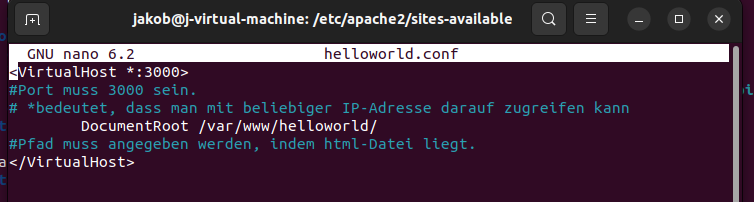
\includegraphics [width = 10 cm] {helloworldConf.png}\\
\\
Aussehen:\\
Der virtuelle host wurde in /etc/apache2/sites-available gespeichert. Dieses Verzeichnis bietet sich an, da man sich hier im Verzeichnis von apache befindet und der Ordner extra von apache angelegt wurde um Vorlagen f"ur Websites darin zu speichern.\\
Vorteile die Datei hier drin zu speichern: Man kann Konfigurationen an der Website ändern, ohne dass diese direkt angepasst werden. Fehler können dadurch vermieden werden. Man hat ein Verzeichnis, in dem alle Entwürfe, Vorlagen und angewendete Dateien gespeichert werden.\\
\item herausfinden, welche ports beleget sind\\
Befehl:
\begin{verbatim} ss -tuln \end{verbatim}
\item Damit man auf einen bestimmten port des Webservers zugreifen kann, muss der Webserver erst wissen, "uber welchen port wir zugreifen wollen. Dementsprechend muss apache diesen Port abh"oren. Dies kann man in den Konfigurationsdateien von apache "andern.\\
Die Datei, die angibt, welchen Ports gelauscht wird findet sich in /etc/apache2
\begin{verbatim}cd /etc/apache2\end{verbatim}
Datei muss mit root rechten bearbeitet werden:
\begin{verbatim}sudo nano ports.conf\end{verbatim}
Port wurde ge"ander in Port 3000 (Listen 3000).
\item Nun muss apache auch Daten des ports verarbeiten k"onnen. Deshalb muss das im virtuellen host auch angepasst/angegeben werden. (siehe oberes Bild)
\item Damit der virtuelle host von apache erkannt und ausgeführt wird und der Webserver gehostet wird, muss man ihn in /etc/apache2/sites-enabled "`kopieren"'. Hierf"ur reicht ein symbolischer Link jedoch aus.\\
Befehle:\\
sudo a2ensite helloworld\\
Dieser Befehl steht f"ur "`Apache 2 Enable site"'. Damit werden automatisch symbolische Links in sites-enabled erstellt, was sehr komfortabel ist.\\
sudo a2dissite helloworld
Mit diesem Befehl werden die symbolischen Links wieder aus sites-enabled entfernt.
\item Firewall muss akzeptieren, dass "uber den port 3000 anfragen auf den Server kommen. 
Befehl: sudo ufw allow 3000\\
tcp und udp protokolle werden hiermit erlaubt $\Rightarrow$ sind Komunikationsprotokolle\\
Mit Hilfe von sudo ufw status wird nun ausgegeben, dass der port f"ur anfragen von außen ge"offnet ist.\\
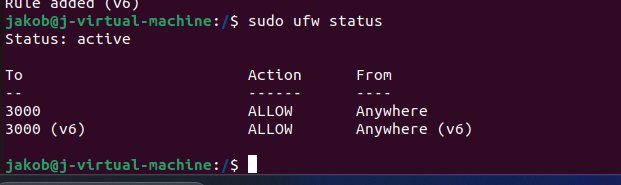
\includegraphics [width = 10 cm] {Status-Firewall.png}
\item apache muss neu gestartet werden, damit "Anderungen in den Konfigurationsdateien angewendet werden.
\begin{verbatim}sudo systemctl restart apache2\end{verbatim}
\item Der Server kann nun mit der IP-Adresse und dem port 3000 aufgerufen werden.
Herausfinden der IP-Adresse: 
\begin{verbatim}hostname -I\end{verbatim}
Zugriff auf Webserver via browser mit 192.168.159.128:3000
\end{enumerate}

\subsection{html Dokument erstellen}
\begin{enumerate}
\item Man muss das Dokument im richtigen Ordner speichern, sodass Apache darauf zugreifen kann:\\
Directory : /var/www\\
Neuer Ordner und neue HTML-Datei: 
\begin{verbatim}
mkdir helloworld
sudo nano index.html
\end{verbatim}
Es ist wichtig, dass man die Datei "`index"' benannt wird, ansonsten wird sie nicht richtig angezeigt.
\item Man muss nun den virtuellen host so anpassen, damit er auf das richtige html-Dokument zugreift. Man muss die Adresse in dem Dokument "andern:\\
Directory: /etc/apache2/sites-available\\
Befehl: 
\begin{verbatim}sudo nano helloworld.conf\end{verbatim}
\item Einf"ugen eines Bildes: Wenn man ein Bild einf"ugen m"ochte verwendet man den relativen Pfadnamen, deshalb ist es hilfreich, wenn man das Bild im selben Verzeichnis oder in einem Unterverzeichnis der html Datei anlegt.
\end{enumerate}
HTML-Datei:\\
\\
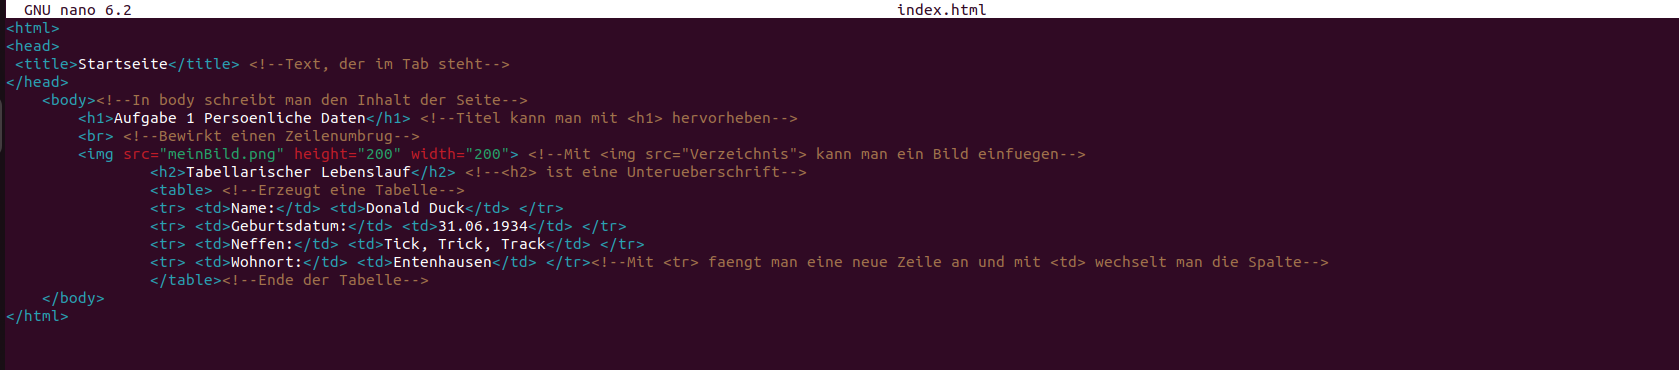
\includegraphics [width = 15 cm] {HTML1.png}
\newpage 
\noindent Website:\\
\\
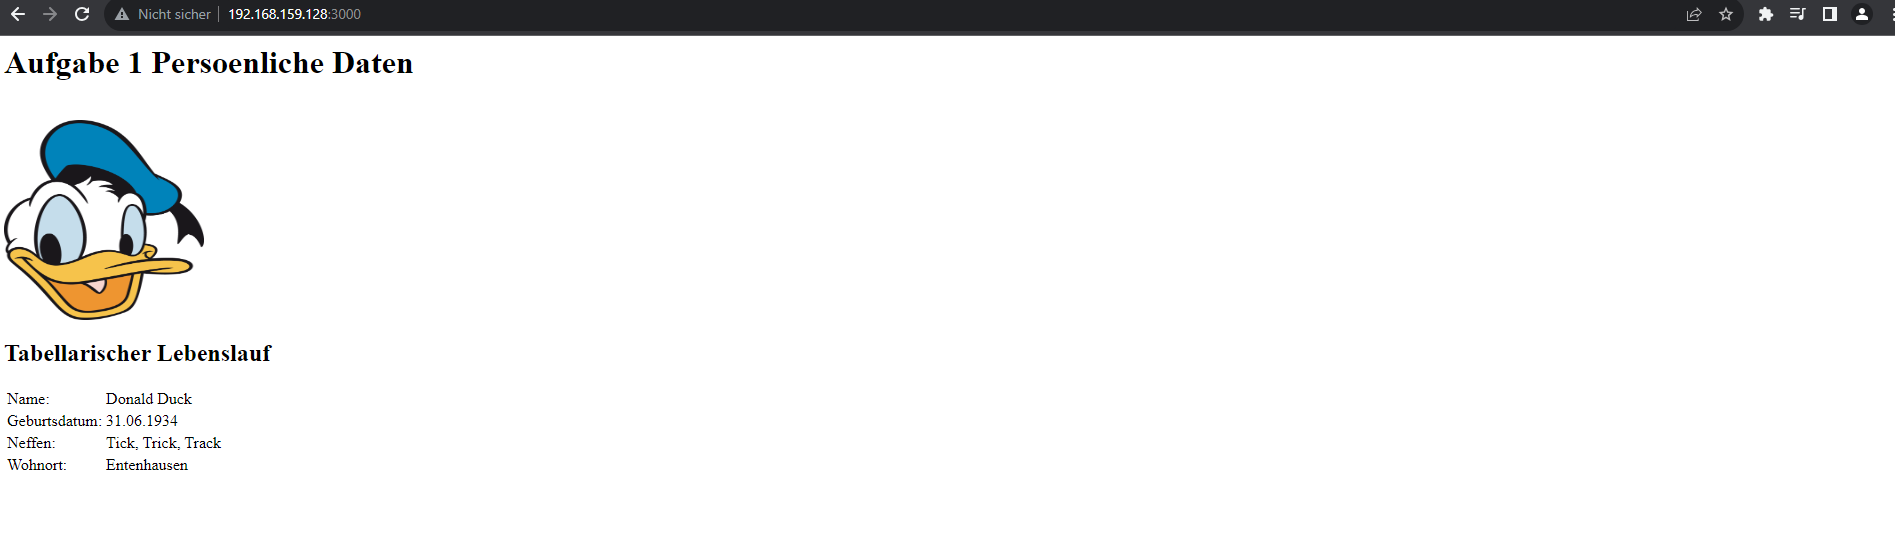
\includegraphics [width = 15 cm] {Website-Aufgabe1.png}\\
\section{Python und Matplotlib}
\subsection{Python}
Python 3 ist in einer Ubuntu-Standardinstallation bereits enthalten, da auch Systemkomponenten Python als Voraussetzung benötigen.\\
Befehl f"ur Version von Python: 
\begin{verbatim}python3 -V\end{verbatim}
\subsection{Matplotlib}
Matplotlib ist eine Programmbibliothek f"ur die Programmiersprache Python. Mit matplotlib lassen sich mathematische Darstellungen anfertigen (bspw. Graphen, Diagramme, ...)
Matplotlib ist kostenlos, frei und quelloffen.\\
\subsection{NumPy}
NumPy ist eine Programmbibliothek f"ur die Programmiersprache Python. NumPy erweitert Python um Funktionen f"ur wissenschaftliches Rechnen und numerische Berechnungen. (erm"oglicht effizientes Rechnen mit Matrizen, mehrdimensionalen Array und Verktoren). NumPy steht f"ur "`Numeric Python"'. NumPy ist kostenlos, frei und quelloffen.\\
\subsection{Installation}
F"ur die Installation von Python Bibliotheken und Paketen ist der Python-Paketmanager (pip) am besten geeignet. Dieser enth"alt viele Pakete spezifisch f"ur Python.
Installation von pip: 
\begin{verbatim}sudo apt install python3-pip \end{verbatim}
Installation von matplotlib mittels pip: 
\begin{verbatim}pip install matplotlib \end{verbatim}
Installation von NumPy mittels pip: 
\begin{verbatim}pip install numpy\end{verbatim}
\subsection{Python Dokument anlegen}
Befehl: 
\begin{verbatim}nano uebung4Grafik.py\end{verbatim}
Programm:\\
\lstinputlisting[style=python]{Grafik.py}
\subsection{Erstellen von requirements.txt}
Dient dazu, eine konsistente Entwicklungsumgebung zu erstellen, in dem die genauen Versionen der Python Pakete darin festgelegt sind.
Andere Entwickler k"onnen dadurch schnell an Projekt weiterarbeiten, da sie leicht die gleichen Pakete herunterladen k"onnen.\\
Version der Pakete herausfinden: 
\begin{verbatim}pip list\end{verbatim}
Datei erstellen: 
\begin{verbatim}nano requirements.txt\end{verbatim}
Alle Pakete herunterladen durch: 
\begin{verbatim}pip install -r requirements.txt\end{verbatim}
Inhalt der Datei:\\
\\
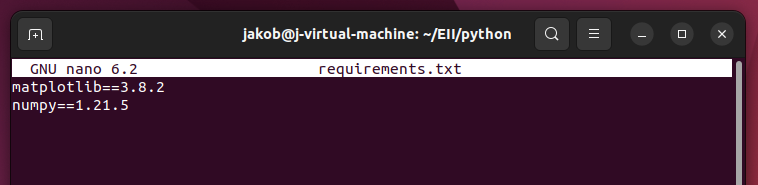
\includegraphics [width = 15 cm] {requirements.png}
\subsection{Automatisierung der Installation und Ausf"uhrung}
Verzeichnis: ~/EII/python
Befehl: 
\begin{verbatim}nano SartGrafik.sh\end{verbatim}
Dateiberechtigungen vergeben und Skript ausf"uhrbar machen: 
\begin{verbatim}chmod +x StartGrafik.sh\end{verbatim}
Skript ausf"uhren: ./StartGrafik.sh
Man muss nun einem Kollegen das Programm, die Bash-Datei und die requirements.txt-Datei geben. Wenn er das Skript ausf"uhrt werden die notwendigen Bibliotheken heruntergeladen und das Programm ausgefu"uhrt.\\
Wichtig ist, dass der Rechner des Kollegen pip und python3 installiert hat.\\
Bash-Skript:\\
\\

\includegraphics [width = 15 cm] {Bash-Skript.png}\\

\subsection{Modifizierte Homepage}
Bild in richtiges Verzeichnis verschieben: 
\begin{verbatim}sudo mv ./Grafik.png /var/www/helloworld \end{verbatim}
Bild der Homepage:\\
\\
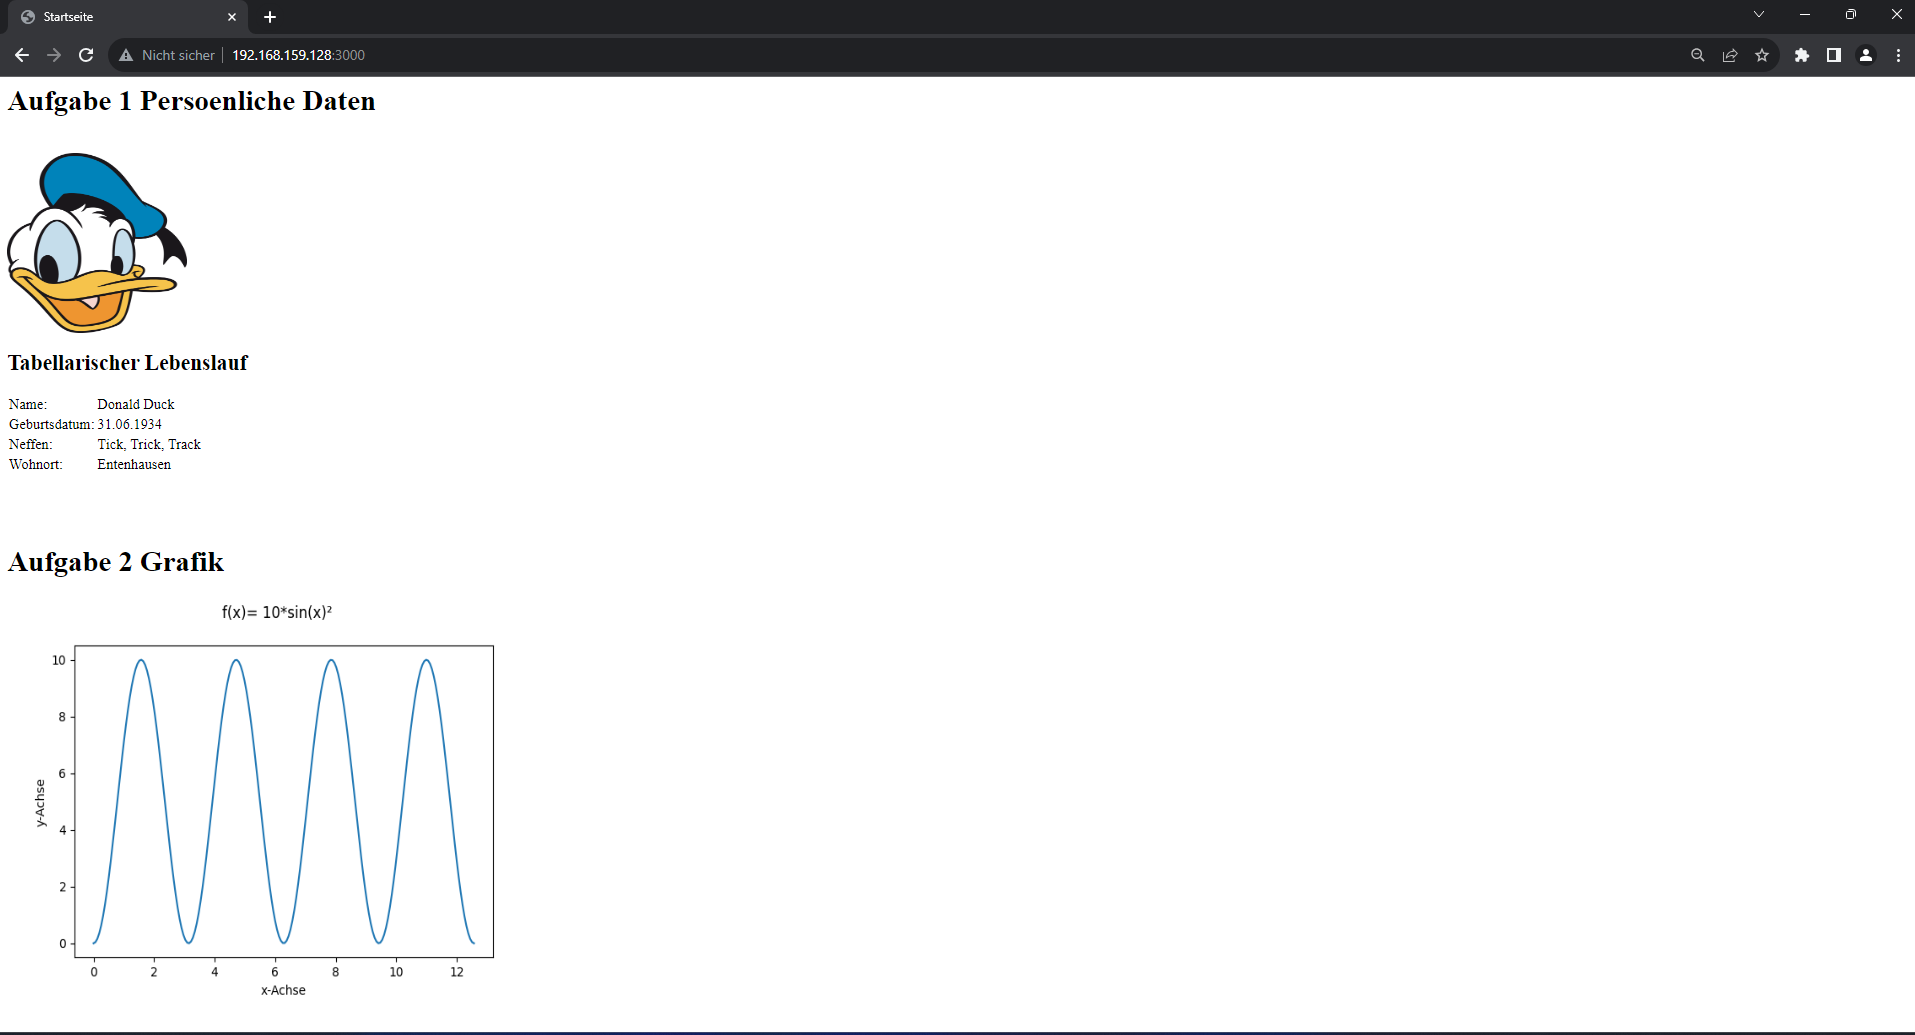
\includegraphics [width = 15 cm] {Website-Aufgabe2.png}
\end{document}
